\documentclass[1p]{elsarticle_modified}
%\bibliographystyle{elsarticle-num}

%\usepackage[colorlinks]{hyperref}
%\usepackage{abbrmath_seonhwa} %\Abb, \Ascr, \Acal ,\Abf, \Afrak
\usepackage{amsfonts}
\usepackage{amssymb}
\usepackage{amsmath}
\usepackage{amsthm}
\usepackage{scalefnt}
\usepackage{amsbsy}
\usepackage{kotex}
\usepackage{caption}
\usepackage{subfig}
\usepackage{color}
\usepackage{graphicx}
\usepackage{xcolor} %% white, black, red, green, blue, cyan, magenta, yellow
\usepackage{float}
\usepackage{setspace}
\usepackage{hyperref}

\usepackage{tikz}
\usetikzlibrary{arrows}

\usepackage{multirow}
\usepackage{array} % fixed length table
\usepackage{hhline}

%%%%%%%%%%%%%%%%%%%%%
\makeatletter
\renewcommand*\env@matrix[1][\arraystretch]{%
	\edef\arraystretch{#1}%
	\hskip -\arraycolsep
	\let\@ifnextchar\new@ifnextchar
	\array{*\c@MaxMatrixCols c}}
\makeatother %https://tex.stackexchange.com/questions/14071/how-can-i-increase-the-line-spacing-in-a-matrix
%%%%%%%%%%%%%%%

\usepackage[normalem]{ulem}

\newcommand{\msout}[1]{\ifmmode\text{\sout{\ensuremath{#1}}}\else\sout{#1}\fi}
%SOURCE: \msout is \stkout macro in https://tex.stackexchange.com/questions/20609/strikeout-in-math-mode

\newcommand{\cancel}[1]{
	\ifmmode
	{\color{red}\msout{#1}}
	\else
	{\color{red}\sout{#1}}
	\fi
}

\newcommand{\add}[1]{
	{\color{blue}\uwave{#1}}
}

\newcommand{\replace}[2]{
	\ifmmode
	{\color{red}\msout{#1}}{\color{blue}\uwave{#2}}
	\else
	{\color{red}\sout{#1}}{\color{blue}\uwave{#2}}
	\fi
}

\newcommand{\Sol}{\mathcal{S}} %segment
\newcommand{\D}{D} %diagram
\newcommand{\A}{\mathcal{A}} %arc


%%%%%%%%%%%%%%%%%%%%%%%%%%%%%5 test

\def\sl{\operatorname{\textup{SL}}(2,\Cbb)}
\def\psl{\operatorname{\textup{PSL}}(2,\Cbb)}
\def\quan{\mkern 1mu \triangleright \mkern 1mu}

\theoremstyle{definition}
\newtheorem{thm}{Theorem}[section]
\newtheorem{prop}[thm]{Proposition}
\newtheorem{lem}[thm]{Lemma}
\newtheorem{ques}[thm]{Question}
\newtheorem{cor}[thm]{Corollary}
\newtheorem{defn}[thm]{Definition}
\newtheorem{exam}[thm]{Example}
\newtheorem{rmk}[thm]{Remark}
\newtheorem{alg}[thm]{Algorithm}

\newcommand{\I}{\sqrt{-1}}
\begin{document}

%\begin{frontmatter}
%
%\title{Boundary parabolic representations of knots up to 8 crossings}
%
%%% Group authors per affiliation:
%\author{Yunhi Cho} 
%\address{Department of Mathematics, University of Seoul, Seoul, Korea}
%\ead{yhcho@uos.ac.kr}
%
%
%\author{Seonhwa Kim} %\fnref{s_kim}}
%\address{Center for Geometry and Physics, Institute for Basic Science, Pohang, 37673, Korea}
%\ead{ryeona17@ibs.re.kr}
%
%\author{Hyuk Kim}
%\address{Department of Mathematical Sciences, Seoul National University, Seoul 08826, Korea}
%\ead{hyukkim@snu.ac.kr}
%
%\author{Seokbeom Yoon}
%\address{Department of Mathematical Sciences, Seoul National University, Seoul, 08826,  Korea}
%\ead{sbyoon15@snu.ac.kr}
%
%\begin{abstract}
%We find all boundary parabolic representation of knots up to 8 crossings.
%
%\end{abstract}
%\begin{keyword}
%    \MSC[2010] 57M25 
%\end{keyword}
%
%\end{frontmatter}

%\linenumbers
%\tableofcontents
%
\newcommand\colored[1]{\textcolor{white}{\rule[-0.35ex]{0.8em}{1.4ex}}\kern-0.8em\color{red} #1}%
%\newcommand\colored[1]{\textcolor{white}{ #1}\kern-2.17ex	\textcolor{white}{ #1}\kern-1.81ex	\textcolor{white}{ #1}\kern-2.15ex\color{red}#1	}

{\Large $\underline{12a_{0381}~(K12a_{0381})}$}

\setlength{\tabcolsep}{10pt}
\renewcommand{\arraystretch}{1.6}
\vspace{1cm}\begin{tabular}{m{100pt}>{\centering\arraybackslash}m{274pt}}
\multirow{5}{120pt}{
	\centering
	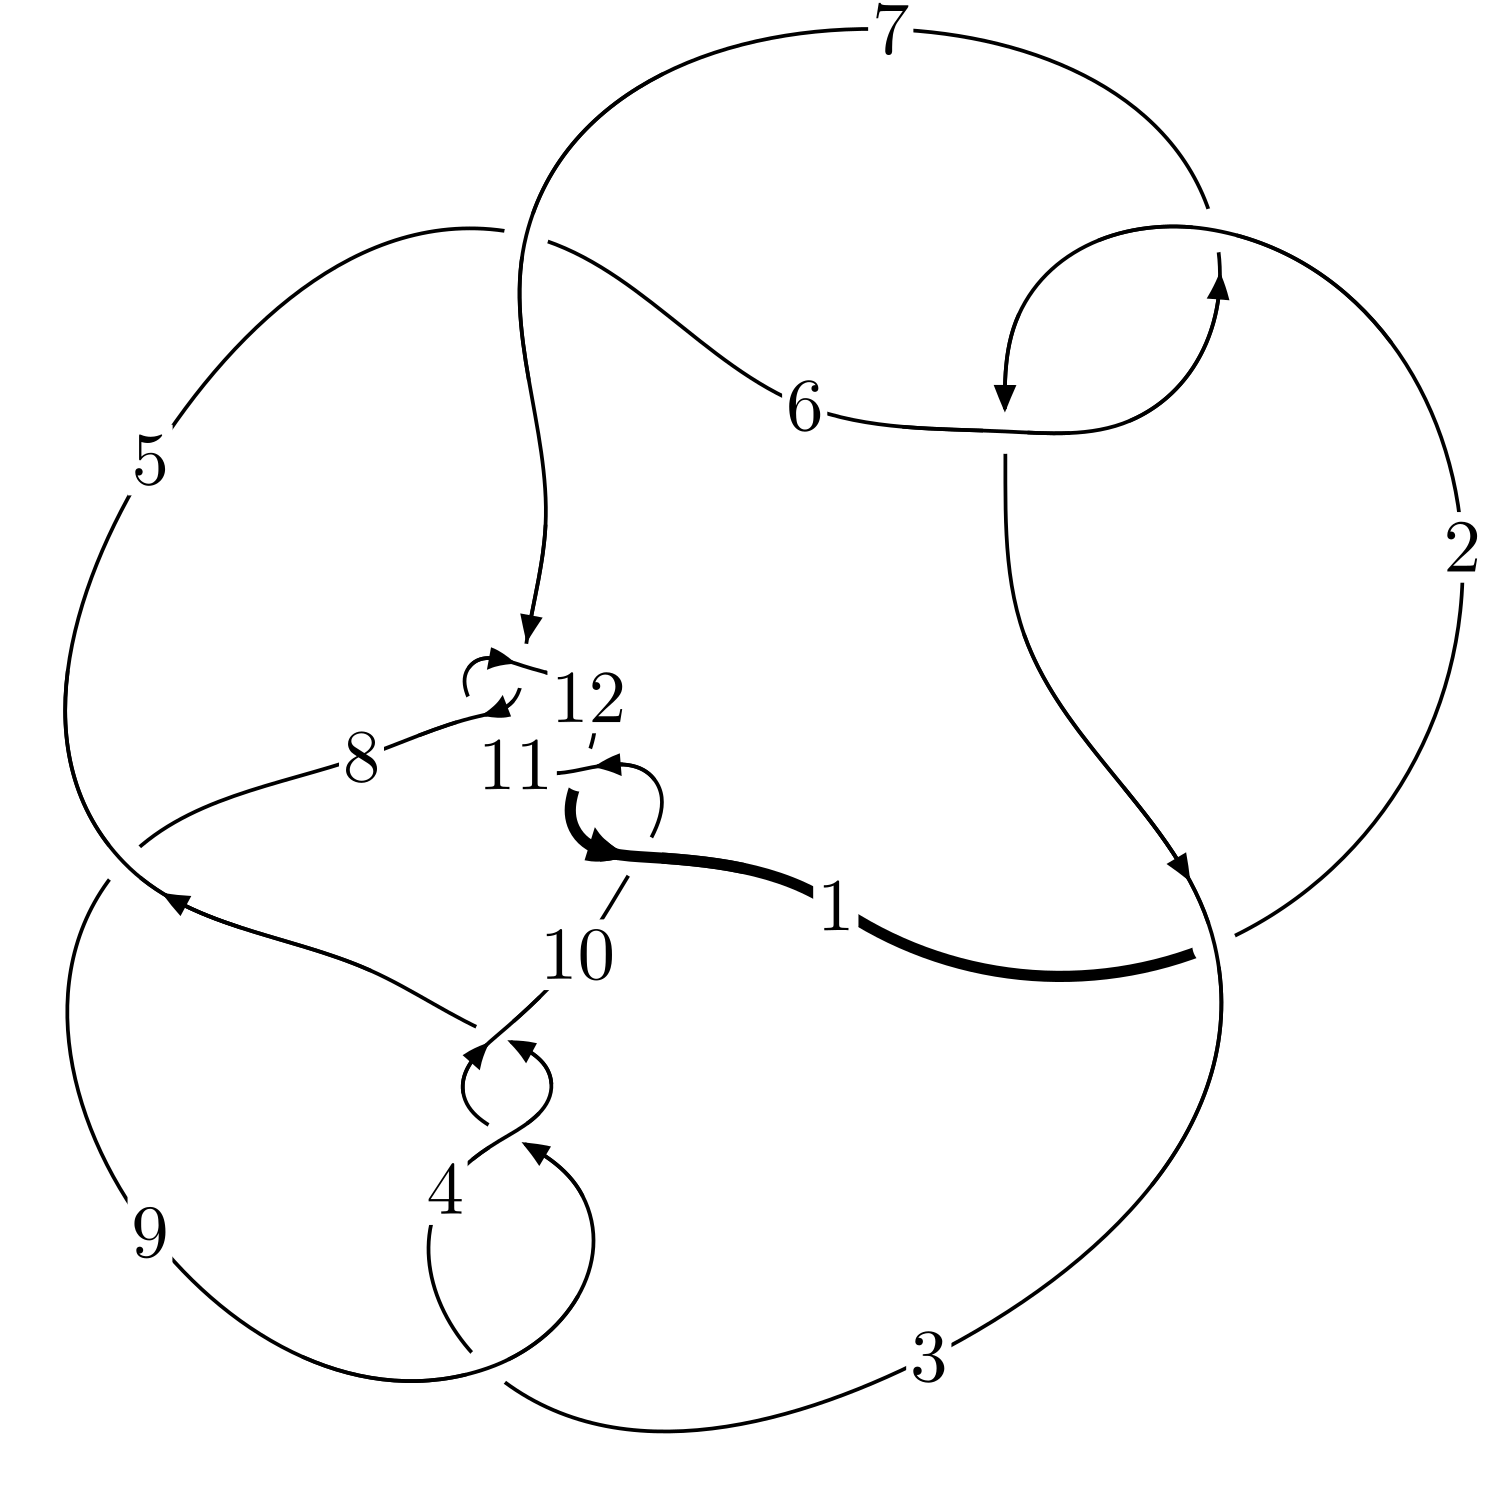
\includegraphics[width=112pt]{../../../GIT/diagram.site/Diagrams/png/1182_12a_0381.png}\\
\ \ \ A knot diagram\footnotemark}&
\allowdisplaybreaks
\textbf{Linearized knot diagam} \\
\cline{2-2}
 &
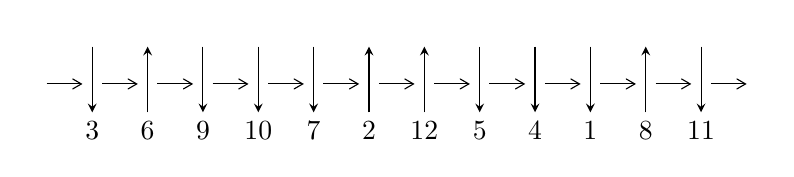
\begin{tikzpicture}[x=20pt, y=17pt]
	% nodes
	\node (C0) at (0, 0) {};
	\node (C1) at (1, 0) {};
	\node (C1U) at (1, +1) {};
	\node (C1D) at (1, -1) {3};

	\node (C2) at (2, 0) {};
	\node (C2U) at (2, +1) {};
	\node (C2D) at (2, -1) {6};

	\node (C3) at (3, 0) {};
	\node (C3U) at (3, +1) {};
	\node (C3D) at (3, -1) {9};

	\node (C4) at (4, 0) {};
	\node (C4U) at (4, +1) {};
	\node (C4D) at (4, -1) {10};

	\node (C5) at (5, 0) {};
	\node (C5U) at (5, +1) {};
	\node (C5D) at (5, -1) {7};

	\node (C6) at (6, 0) {};
	\node (C6U) at (6, +1) {};
	\node (C6D) at (6, -1) {2};

	\node (C7) at (7, 0) {};
	\node (C7U) at (7, +1) {};
	\node (C7D) at (7, -1) {12};

	\node (C8) at (8, 0) {};
	\node (C8U) at (8, +1) {};
	\node (C8D) at (8, -1) {5};

	\node (C9) at (9, 0) {};
	\node (C9U) at (9, +1) {};
	\node (C9D) at (9, -1) {4};

	\node (C10) at (10, 0) {};
	\node (C10U) at (10, +1) {};
	\node (C10D) at (10, -1) {1};

	\node (C11) at (11, 0) {};
	\node (C11U) at (11, +1) {};
	\node (C11D) at (11, -1) {8};

	\node (C12) at (12, 0) {};
	\node (C12U) at (12, +1) {};
	\node (C12D) at (12, -1) {11};
	\node (C13) at (13, 0) {};

	% arrows
	\draw[->,>={angle 60}]
	(C0) edge (C1) (C1) edge (C2) (C2) edge (C3) (C3) edge (C4) (C4) edge (C5) (C5) edge (C6) (C6) edge (C7) (C7) edge (C8) (C8) edge (C9) (C9) edge (C10) (C10) edge (C11) (C11) edge (C12) (C12) edge (C13) ;	\draw[->,>=stealth]
	(C1U) edge (C1D) (C2D) edge (C2U) (C3U) edge (C3D) (C4U) edge (C4D) (C5U) edge (C5D) (C6D) edge (C6U) (C7D) edge (C7U) (C8U) edge (C8D) (C9U) edge (C9D) (C10U) edge (C10D) (C11D) edge (C11U) (C12U) edge (C12D) ;
	\end{tikzpicture} \\
\hhline{~~} \\& 
\textbf{Solving Sequence} \\ \cline{2-2} 
 &
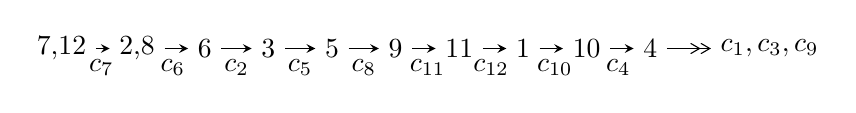
\begin{tikzpicture}[x=23pt, y=7pt]
	% node
	\node (A0) at (-1/8, 0) {7,12};
	\node (A1) at (17/16, 0) {2,8};
	\node (A2) at (17/8, 0) {6};
	\node (A3) at (25/8, 0) {3};
	\node (A4) at (33/8, 0) {5};
	\node (A5) at (41/8, 0) {9};
	\node (A6) at (49/8, 0) {11};
	\node (A7) at (57/8, 0) {1};
	\node (A8) at (65/8, 0) {10};
	\node (A9) at (73/8, 0) {4};
	\node (C1) at (1/2, -1) {$c_{7}$};
	\node (C2) at (13/8, -1) {$c_{6}$};
	\node (C3) at (21/8, -1) {$c_{2}$};
	\node (C4) at (29/8, -1) {$c_{5}$};
	\node (C5) at (37/8, -1) {$c_{8}$};
	\node (C6) at (45/8, -1) {$c_{11}$};
	\node (C7) at (53/8, -1) {$c_{12}$};
	\node (C8) at (61/8, -1) {$c_{10}$};
	\node (C9) at (69/8, -1) {$c_{4}$};
	\node (A10) at (11, 0) {$c_{1},c_{3},c_{9}$};

	% edge
	\draw[->,>=stealth]	
	(A0) edge (A1) (A1) edge (A2) (A2) edge (A3) (A3) edge (A4) (A4) edge (A5) (A5) edge (A6) (A6) edge (A7) (A7) edge (A8) (A8) edge (A9) ;
	\draw[->>,>={angle 60}]	
	(A9) edge (A10);
\end{tikzpicture} \\ 

\end{tabular} \\

\footnotetext{
The image of knot diagram is generated by the software ``\textbf{Draw programme}" developed by Andrew Bartholomew(\url{http://www.layer8.co.uk/maths/draw/index.htm\#Running-draw}), where we modified some parts for our purpose(\url{https://github.com/CATsTAILs/LinksPainter}).
}\phantom \\ \newline 
\centering \textbf{Ideals for irreducible components\footnotemark of $X_{\text{par}}$} 
 
\begin{align*}
I^u_{1}&=\langle 
b- u,\;u^{22}- u^{21}+\cdots+2 a+u,\;u^{23}- u^{22}+\cdots+4 u^2+1\rangle \\
I^u_{2}&=\langle 
-1.58008\times10^{30} u^{65}+4.09523\times10^{30} u^{64}+\cdots+2.14580\times10^{30} b+1.44290\times10^{31},\\
\phantom{I^u_{2}}&\phantom{= \langle  }-1.35351\times10^{31} u^{65}+4.37094\times10^{31} u^{64}+\cdots+3.00412\times10^{31} a-1.14573\times10^{30},\\
\phantom{I^u_{2}}&\phantom{= \langle  }u^{66}-2 u^{65}+\cdots+19 u+7\rangle \\
I^u_{3}&=\langle 
b+u,\;a^2+2 a u-4 a-3 u+1,\;u^2- u+1\rangle \\
I^u_{4}&=\langle 
b+u,\;a+u+2,\;u^2+u+1\rangle \\
I^u_{5}&=\langle 
b- u+1,\;a^2+2 u,\;u^2- u+1\rangle \\
I^u_{6}&=\langle 
b- u-1,\;a,\;u^2+u+1\rangle \\
\\
\end{align*}
\raggedright * 6 irreducible components of $\dim_{\mathbb{C}}=0$, with total 101 representations.\\
\footnotetext{All coefficients of polynomials are rational numbers. But the coefficients are sometimes approximated in decimal forms when there is not enough margin.}
\newpage
\renewcommand{\arraystretch}{1}
\centering \section*{I. $I^u_{1}= \langle b- u,\;u^{22}- u^{21}+\cdots+2 a+u,\;u^{23}- u^{22}+\cdots+4 u^2+1 \rangle$}
\flushleft \textbf{(i) Arc colorings}\\
\begin{tabular}{m{7pt} m{180pt} m{7pt} m{180pt} }
\flushright $a_{7}=$&$\begin{pmatrix}1\\0\end{pmatrix}$ \\
\flushright $a_{12}=$&$\begin{pmatrix}0\\u\end{pmatrix}$ \\
\flushright $a_{2}=$&$\begin{pmatrix}-\frac{1}{2} u^{22}+\frac{1}{2} u^{21}+\cdots-4 u^3-\frac{1}{2} u\\u\end{pmatrix}$ \\
\flushright $a_{8}=$&$\begin{pmatrix}1\\- u^2\end{pmatrix}$ \\
\flushright $a_{6}=$&$\begin{pmatrix}\frac{1}{2} u^{19}-\frac{1}{2} u^{18}+\cdots+\frac{3}{2} u^2+\frac{3}{2}\\u^2\end{pmatrix}$ \\
\flushright $a_{3}=$&$\begin{pmatrix}-\frac{1}{2} u^{22}+\frac{1}{2} u^{21}+\cdots-\frac{5}{2} u^3+u\\u^3+u\end{pmatrix}$ \\
\flushright $a_{5}=$&$\begin{pmatrix}\frac{1}{2} u^{19}-\frac{1}{2} u^{18}+\cdots+\frac{5}{2} u^2+\frac{3}{2}\\u^2\end{pmatrix}$ \\
\flushright $a_{9}=$&$\begin{pmatrix}-\frac{1}{2} u^{22}+u^{21}+\cdots+2 u^2+\frac{1}{2}\\-\frac{1}{2} u^{21}+\frac{1}{2} u^{20}+\cdots-3 u^2-\frac{1}{2}\end{pmatrix}$ \\
\flushright $a_{11}=$&$\begin{pmatrix}- u\\u^3+u\end{pmatrix}$ \\
\flushright $a_{1}=$&$\begin{pmatrix}- u^3\\u^5+u^3+u\end{pmatrix}$ \\
\flushright $a_{10}=$&$\begin{pmatrix}- u^5- u\\u^7+u^5+2 u^3+u\end{pmatrix}$ \\
\flushright $a_{4}=$&$\begin{pmatrix}\frac{1}{2} u^{21}-\frac{1}{2} u^{20}+\cdots+4 u^2+\frac{3}{2}\\\frac{1}{2} u^{21}-\frac{1}{2} u^{20}+\cdots+2 u^2+\frac{1}{2}\end{pmatrix}$\\&\end{tabular}
\flushleft \textbf{(ii) Obstruction class $= -1$}\\~\\
\flushleft \textbf{(iii) Cusp Shapes $= -5 u^{22}+3 u^{21}-16 u^{20}+6 u^{19}-53 u^{18}+17 u^{17}-101 u^{16}+17 u^{15}-174 u^{14}+7 u^{13}-224 u^{12}-20 u^{11}-239 u^{10}-75 u^9-209 u^8-97 u^7-132 u^6-106 u^5-73 u^4-72 u^3-27 u^2-17 u-9$}\\~\\
\newpage\renewcommand{\arraystretch}{1}
\flushleft \textbf{(iv) u-Polynomials at the component}\newline \\
\begin{tabular}{m{50pt}|m{274pt}}
Crossings & \hspace{64pt}u-Polynomials at each crossing \\
\hline $$\begin{aligned}c_{1},c_{5},c_{10}\\c_{12}\end{aligned}$$&$\begin{aligned}
&u^{23}+7 u^{22}+\cdots-8 u-1
\end{aligned}$\\
\hline $$\begin{aligned}c_{2},c_{6},c_{7}\\c_{11}\end{aligned}$$&$\begin{aligned}
&u^{23}- u^{22}+\cdots+4 u^2+1
\end{aligned}$\\
\hline $$\begin{aligned}c_{3},c_{4},c_{9}\end{aligned}$$&$\begin{aligned}
&u^{23}+5 u^{22}+\cdots+4 u+4
\end{aligned}$\\
\hline $$\begin{aligned}c_{8}\end{aligned}$$&$\begin{aligned}
&u^{23}-15 u^{22}+\cdots+2004 u-332
\end{aligned}$\\
\hline
\end{tabular}\\~\\
\newpage\renewcommand{\arraystretch}{1}
\flushleft \textbf{(v) Riley Polynomials at the component}\newline \\
\begin{tabular}{m{50pt}|m{274pt}}
Crossings & \hspace{64pt}Riley Polynomials at each crossing \\
\hline $$\begin{aligned}c_{1},c_{5},c_{10}\\c_{12}\end{aligned}$$&$\begin{aligned}
&y^{23}+23 y^{22}+\cdots-4 y-1
\end{aligned}$\\
\hline $$\begin{aligned}c_{2},c_{6},c_{7}\\c_{11}\end{aligned}$$&$\begin{aligned}
&y^{23}+7 y^{22}+\cdots-8 y-1
\end{aligned}$\\
\hline $$\begin{aligned}c_{3},c_{4},c_{9}\end{aligned}$$&$\begin{aligned}
&y^{23}-21 y^{22}+\cdots-48 y-16
\end{aligned}$\\
\hline $$\begin{aligned}c_{8}\end{aligned}$$&$\begin{aligned}
&y^{23}- y^{22}+\cdots+356048 y-110224
\end{aligned}$\\
\hline
\end{tabular}\\~\\
\newpage\flushleft \textbf{(vi) Complex Volumes and Cusp Shapes}
$$\begin{array}{c|c|c}  
\text{Solutions to }I^u_{1}& \I (\text{vol} + \sqrt{-1}CS) & \text{Cusp shape}\\
 \hline 
\begin{aligned}
u &= -0.108766 + 1.038960 I \\
a &= -0.14445 + 2.16071 I \\
b &= -0.108766 + 1.038960 I\end{aligned}
 & -9.31458 - 4.23664 I & -14.9374 + 4.2518 I \\ \hline\begin{aligned}
u &= -0.108766 - 1.038960 I \\
a &= -0.14445 - 2.16071 I \\
b &= -0.108766 - 1.038960 I\end{aligned}
 & -9.31458 + 4.23664 I & -14.9374 - 4.2518 I \\ \hline\begin{aligned}
u &= \phantom{-}0.062381 + 0.953110 I \\
a &= \phantom{-}0.17223 + 1.91880 I \\
b &= \phantom{-}0.062381 + 0.953110 I\end{aligned}
 & -3.67662 + 1.63978 I & -11.45625 - 4.68535 I \\ \hline\begin{aligned}
u &= \phantom{-}0.062381 - 0.953110 I \\
a &= \phantom{-}0.17223 - 1.91880 I \\
b &= \phantom{-}0.062381 - 0.953110 I\end{aligned}
 & -3.67662 - 1.63978 I & -11.45625 + 4.68535 I \\ \hline\begin{aligned}
u &= \phantom{-}0.878988 + 0.705166 I \\
a &= -1.38624 - 0.52383 I \\
b &= \phantom{-}0.878988 + 0.705166 I\end{aligned}
 & \phantom{-}4.20055 - 4.17420 I & -1.40540 + 0.69157 I \\ \hline\begin{aligned}
u &= \phantom{-}0.878988 - 0.705166 I \\
a &= -1.38624 + 0.52383 I \\
b &= \phantom{-}0.878988 - 0.705166 I\end{aligned}
 & \phantom{-}4.20055 + 4.17420 I & -1.40540 - 0.69157 I \\ \hline\begin{aligned}
u &= -0.709127 + 0.898384 I \\
a &= \phantom{-}3.06567 - 0.32207 I \\
b &= -0.709127 + 0.898384 I\end{aligned}
 & -2.78113 - 5.44900 I & -3.47285 + 6.34023 I \\ \hline\begin{aligned}
u &= -0.709127 - 0.898384 I \\
a &= \phantom{-}3.06567 + 0.32207 I \\
b &= -0.709127 - 0.898384 I\end{aligned}
 & -2.78113 + 5.44900 I & -3.47285 - 6.34023 I \\ \hline\begin{aligned}
u &= -0.868691 + 0.769532 I \\
a &= \phantom{-}1.60761 - 0.45900 I \\
b &= -0.868691 + 0.769532 I\end{aligned}
 & \phantom{-}9.09763 - 0.31187 I & \phantom{-}2.24462 + 1.40830 I \\ \hline\begin{aligned}
u &= -0.868691 - 0.769532 I \\
a &= \phantom{-}1.60761 + 0.45900 I \\
b &= -0.868691 - 0.769532 I\end{aligned}
 & \phantom{-}9.09763 + 0.31187 I & \phantom{-}2.24462 - 1.40830 I\\
 \hline 
 \end{array}$$\newpage$$\begin{array}{c|c|c}  
\text{Solutions to }I^u_{1}& \I (\text{vol} + \sqrt{-1}CS) & \text{Cusp shape}\\
 \hline 
\begin{aligned}
u &= \phantom{-}0.838998 + 0.838326 I \\
a &= -1.91420 - 0.34412 I \\
b &= \phantom{-}0.838998 + 0.838326 I\end{aligned}
 & \phantom{-}6.46982 + 5.13305 I & -0.60159 - 5.77161 I \\ \hline\begin{aligned}
u &= \phantom{-}0.838998 - 0.838326 I \\
a &= -1.91420 + 0.34412 I \\
b &= \phantom{-}0.838998 - 0.838326 I\end{aligned}
 & \phantom{-}6.46982 - 5.13305 I & -0.60159 + 5.77161 I \\ \hline\begin{aligned}
u &= \phantom{-}0.780652 + 0.967249 I \\
a &= -2.39587 + 0.31250 I \\
b &= \phantom{-}0.780652 + 0.967249 I\end{aligned}
 & \phantom{-}5.63176 + 7.01945 I & -1.80788 - 4.37801 I \\ \hline\begin{aligned}
u &= \phantom{-}0.780652 - 0.967249 I \\
a &= -2.39587 - 0.31250 I \\
b &= \phantom{-}0.780652 - 0.967249 I\end{aligned}
 & \phantom{-}5.63176 - 7.01945 I & -1.80788 + 4.37801 I \\ \hline\begin{aligned}
u &= -0.320435 + 0.678319 I \\
a &= -1.41963 + 0.05223 I \\
b &= -0.320435 + 0.678319 I\end{aligned}
 & -5.40470 - 2.53254 I & -9.43035 + 2.23223 I \\ \hline\begin{aligned}
u &= -0.320435 - 0.678319 I \\
a &= -1.41963 - 0.05223 I \\
b &= -0.320435 - 0.678319 I\end{aligned}
 & -5.40470 + 2.53254 I & -9.43035 - 2.23223 I \\ \hline\begin{aligned}
u &= -0.770543 + 1.018970 I \\
a &= \phantom{-}2.33411 + 0.64664 I \\
b &= -0.770543 + 1.018970 I\end{aligned}
 & \phantom{-}7.50703 - 11.94160 I & -0.51059 + 8.65040 I \\ \hline\begin{aligned}
u &= -0.770543 - 1.018970 I \\
a &= \phantom{-}2.33411 - 0.64664 I \\
b &= -0.770543 - 1.018970 I\end{aligned}
 & \phantom{-}7.50703 + 11.94160 I & -0.51059 - 8.65040 I \\ \hline\begin{aligned}
u &= \phantom{-}0.748511 + 1.049130 I \\
a &= -2.32792 + 0.88202 I \\
b &= \phantom{-}0.748511 + 1.049130 I\end{aligned}
 & \phantom{-}2.0337 + 16.3152 I & -4.71784 - 9.86318 I \\ \hline\begin{aligned}
u &= \phantom{-}0.748511 - 1.049130 I \\
a &= -2.32792 - 0.88202 I \\
b &= \phantom{-}0.748511 - 1.049130 I\end{aligned}
 & \phantom{-}2.0337 - 16.3152 I & -4.71784 + 9.86318 I\\
 \hline 
 \end{array}$$\newpage$$\begin{array}{c|c|c}  
\text{Solutions to }I^u_{1}& \I (\text{vol} + \sqrt{-1}CS) & \text{Cusp shape}\\
 \hline 
\begin{aligned}
u &= -0.538161\phantom{ +0.000000I} \\
a &= \phantom{-}0.226955\phantom{ +0.000000I} \\
b &= -0.538161\phantom{ +0.000000I}\end{aligned}
 & -2.63402\phantom{ +0.000000I} & -1.54930\phantom{ +0.000000I} \\ \hline\begin{aligned}
u &= \phantom{-}0.237113 + 0.441635 I \\
a &= \phantom{-}0.295194 - 0.025537 I \\
b &= \phantom{-}0.237113 + 0.441635 I\end{aligned}
 & -0.109440 + 0.967023 I & -2.12980 - 6.92815 I \\ \hline\begin{aligned}
u &= \phantom{-}0.237113 - 0.441635 I \\
a &= \phantom{-}0.295194 + 0.025537 I \\
b &= \phantom{-}0.237113 - 0.441635 I\end{aligned}
 & -0.109440 - 0.967023 I & -2.12980 + 6.92815 I\\
 \hline 
 \end{array}$$\newpage\newpage\renewcommand{\arraystretch}{1}
\centering \section*{II. $I^u_{2}= \langle -1.58\times10^{30} u^{65}+4.10\times10^{30} u^{64}+\cdots+2.15\times10^{30} b+1.44\times10^{31},\;-1.35\times10^{31} u^{65}+4.37\times10^{31} u^{64}+\cdots+3.00\times10^{31} a-1.15\times10^{30},\;u^{66}-2 u^{65}+\cdots+19 u+7 \rangle$}
\flushleft \textbf{(i) Arc colorings}\\
\begin{tabular}{m{7pt} m{180pt} m{7pt} m{180pt} }
\flushright $a_{7}=$&$\begin{pmatrix}1\\0\end{pmatrix}$ \\
\flushright $a_{12}=$&$\begin{pmatrix}0\\u\end{pmatrix}$ \\
\flushright $a_{2}=$&$\begin{pmatrix}0.450551 u^{65}-1.45498 u^{64}+\cdots+0.601985 u+0.0381388\\0.736361 u^{65}-1.90849 u^{64}+\cdots-17.1039 u-6.72429\end{pmatrix}$ \\
\flushright $a_{8}=$&$\begin{pmatrix}1\\- u^2\end{pmatrix}$ \\
\flushright $a_{6}=$&$\begin{pmatrix}0.880632 u^{65}-0.628257 u^{64}+\cdots+10.5151 u+7.47661\\0.134748 u^{65}-0.326968 u^{64}+\cdots+19.1692 u+3.77720\end{pmatrix}$ \\
\flushright $a_{3}=$&$\begin{pmatrix}0.541655 u^{65}-1.07474 u^{64}+\cdots+13.2018 u+5.03970\\0.859372 u^{65}-2.24529 u^{64}+\cdots+1.06882 u-2.22730\end{pmatrix}$ \\
\flushright $a_{5}=$&$\begin{pmatrix}1.01538 u^{65}-0.955224 u^{64}+\cdots+29.6843 u+11.2538\\0.134748 u^{65}-0.326968 u^{64}+\cdots+19.1692 u+3.77720\end{pmatrix}$ \\
\flushright $a_{9}=$&$\begin{pmatrix}-0.644879 u^{65}+1.15798 u^{64}+\cdots+2.59190 u+1.58917\\-0.317784 u^{65}-0.0128892 u^{64}+\cdots-7.61429 u-2.11502\end{pmatrix}$ \\
\flushright $a_{11}=$&$\begin{pmatrix}- u\\u^3+u\end{pmatrix}$ \\
\flushright $a_{1}=$&$\begin{pmatrix}- u^3\\u^5+u^3+u\end{pmatrix}$ \\
\flushright $a_{10}=$&$\begin{pmatrix}- u^5- u\\u^7+u^5+2 u^3+u\end{pmatrix}$ \\
\flushright $a_{4}=$&$\begin{pmatrix}1.40413 u^{65}-1.90048 u^{64}+\cdots+6.61630 u+4.46567\\0.103837 u^{65}-0.390389 u^{64}+\cdots+18.6949 u+4.37292\end{pmatrix}$\\&\end{tabular}
\flushleft \textbf{(ii) Obstruction class $= -1$}\\~\\
\flushleft \textbf{(iii) Cusp Shapes $= -0.117014 u^{65}+1.08091 u^{64}+\cdots-52.4974 u-13.7114$}\\~\\
\newpage\renewcommand{\arraystretch}{1}
\flushleft \textbf{(iv) u-Polynomials at the component}\newline \\
\begin{tabular}{m{50pt}|m{274pt}}
Crossings & \hspace{64pt}u-Polynomials at each crossing \\
\hline $$\begin{aligned}c_{1},c_{5},c_{10}\\c_{12}\end{aligned}$$&$\begin{aligned}
&u^{66}+22 u^{65}+\cdots+591 u+49
\end{aligned}$\\
\hline $$\begin{aligned}c_{2},c_{6},c_{7}\\c_{11}\end{aligned}$$&$\begin{aligned}
&u^{66}-2 u^{65}+\cdots+19 u+7
\end{aligned}$\\
\hline $$\begin{aligned}c_{3},c_{4},c_{9}\end{aligned}$$&$\begin{aligned}
&(u^{33}-2 u^{32}+\cdots+5 u^3-2)^{2}
\end{aligned}$\\
\hline $$\begin{aligned}c_{8}\end{aligned}$$&$\begin{aligned}
&(u^{33}+6 u^{32}+\cdots+84 u+22)^{2}
\end{aligned}$\\
\hline
\end{tabular}\\~\\
\newpage\renewcommand{\arraystretch}{1}
\flushleft \textbf{(v) Riley Polynomials at the component}\newline \\
\begin{tabular}{m{50pt}|m{274pt}}
Crossings & \hspace{64pt}Riley Polynomials at each crossing \\
\hline $$\begin{aligned}c_{1},c_{5},c_{10}\\c_{12}\end{aligned}$$&$\begin{aligned}
&y^{66}+46 y^{65}+\cdots+47227 y+2401
\end{aligned}$\\
\hline $$\begin{aligned}c_{2},c_{6},c_{7}\\c_{11}\end{aligned}$$&$\begin{aligned}
&y^{66}+22 y^{65}+\cdots+591 y+49
\end{aligned}$\\
\hline $$\begin{aligned}c_{3},c_{4},c_{9}\end{aligned}$$&$\begin{aligned}
&(y^{33}-30 y^{32}+\cdots-72 y^2-4)^{2}
\end{aligned}$\\
\hline $$\begin{aligned}c_{8}\end{aligned}$$&$\begin{aligned}
&(y^{33}+10 y^{32}+\cdots+808 y-484)^{2}
\end{aligned}$\\
\hline
\end{tabular}\\~\\
\newpage\flushleft \textbf{(vi) Complex Volumes and Cusp Shapes}
$$\begin{array}{c|c|c}  
\text{Solutions to }I^u_{2}& \I (\text{vol} + \sqrt{-1}CS) & \text{Cusp shape}\\
 \hline 
\begin{aligned}
u &= \phantom{-}0.780007 + 0.702896 I \\
a &= \phantom{-}0.060274 + 0.274900 I \\
b &= -0.217053 + 1.123410 I\end{aligned}
 & -3.25939 - 4.10922 I & -6.90114 + 3.20990 I \\ \hline\begin{aligned}
u &= \phantom{-}0.780007 - 0.702896 I \\
a &= \phantom{-}0.060274 - 0.274900 I \\
b &= -0.217053 - 1.123410 I\end{aligned}
 & -3.25939 + 4.10922 I & -6.90114 - 3.20990 I \\ \hline\begin{aligned}
u &= -0.711321 + 0.791297 I \\
a &= -0.056822 + 0.187212 I \\
b &= \phantom{-}0.331350 + 1.060870 I\end{aligned}
 & \phantom{-}1.24121 + 0.80287 I & \phantom{-0.000000 } 0 \\ \hline\begin{aligned}
u &= -0.711321 - 0.791297 I \\
a &= -0.056822 - 0.187212 I \\
b &= \phantom{-}0.331350 - 1.060870 I\end{aligned}
 & \phantom{-}1.24121 - 0.80287 I & \phantom{-0.000000 } 0 \\ \hline\begin{aligned}
u &= \phantom{-}0.718922 + 0.797842 I \\
a &= \phantom{-}1.47367 - 0.63983 I \\
b &= -0.435907 - 1.078550 I\end{aligned}
 & -1.97159 + 3.23829 I & -4.00000 - 3.70582 I \\ \hline\begin{aligned}
u &= \phantom{-}0.718922 - 0.797842 I \\
a &= \phantom{-}1.47367 + 0.63983 I \\
b &= -0.435907 + 1.078550 I\end{aligned}
 & -1.97159 - 3.23829 I & -4.00000 + 3.70582 I \\ \hline\begin{aligned}
u &= -0.252240 + 0.890572 I \\
a &= -0.682248 + 0.144403 I \\
b &= -0.442341 + 0.328309 I\end{aligned}
 & -5.30265 - 2.57775 I & -8.82504 + 3.79477 I \\ \hline\begin{aligned}
u &= -0.252240 - 0.890572 I \\
a &= -0.682248 - 0.144403 I \\
b &= -0.442341 - 0.328309 I\end{aligned}
 & -5.30265 + 2.57775 I & -8.82504 - 3.79477 I \\ \hline\begin{aligned}
u &= -0.713764 + 0.843003 I \\
a &= \phantom{-}1.58827 + 1.87585 I \\
b &= -0.713764 - 0.843003 I\end{aligned}
 & -2.60888\phantom{ +0.000000I} & \phantom{-0.000000 } 0 \\ \hline\begin{aligned}
u &= -0.713764 - 0.843003 I \\
a &= \phantom{-}1.58827 - 1.87585 I \\
b &= -0.713764 + 0.843003 I\end{aligned}
 & -2.60888\phantom{ +0.000000I} & \phantom{-0.000000 } 0\\
 \hline 
 \end{array}$$\newpage$$\begin{array}{c|c|c}  
\text{Solutions to }I^u_{2}& \I (\text{vol} + \sqrt{-1}CS) & \text{Cusp shape}\\
 \hline 
\begin{aligned}
u &= \phantom{-}0.587924 + 0.938053 I \\
a &= \phantom{-}1.54849 - 0.69333 I \\
b &= -0.233499 - 0.806742 I\end{aligned}
 & -0.73076 + 3.39395 I & \phantom{-0.000000 } 0 \\ \hline\begin{aligned}
u &= \phantom{-}0.587924 - 0.938053 I \\
a &= \phantom{-}1.54849 + 0.69333 I \\
b &= -0.233499 + 0.806742 I\end{aligned}
 & -0.73076 - 3.39395 I & \phantom{-0.000000 } 0 \\ \hline\begin{aligned}
u &= \phantom{-}0.786418 + 0.782314 I \\
a &= \phantom{-}0.842464 - 0.449392 I \\
b &= -0.769109 + 0.132418 I\end{aligned}
 & \phantom{-}0.933995 - 0.933678 I & \phantom{-0.000000 } 0 \\ \hline\begin{aligned}
u &= \phantom{-}0.786418 - 0.782314 I \\
a &= \phantom{-}0.842464 + 0.449392 I \\
b &= -0.769109 - 0.132418 I\end{aligned}
 & \phantom{-}0.933995 + 0.933678 I & \phantom{-0.000000 } 0 \\ \hline\begin{aligned}
u &= \phantom{-}0.331350 + 1.060870 I \\
a &= -0.181882 + 0.044732 I \\
b &= -0.711321 + 0.791297 I\end{aligned}
 & \phantom{-}1.24121 + 0.80287 I & \phantom{-0.000000 } 0 \\ \hline\begin{aligned}
u &= \phantom{-}0.331350 - 1.060870 I \\
a &= -0.181882 - 0.044732 I \\
b &= -0.711321 - 0.791297 I\end{aligned}
 & \phantom{-}1.24121 - 0.80287 I & \phantom{-0.000000 } 0 \\ \hline\begin{aligned}
u &= \phantom{-}0.884836 + 0.675520 I \\
a &= -1.46006 + 0.36957 I \\
b &= \phantom{-}0.759584 - 1.033520 I\end{aligned}
 & \phantom{-}3.18615 - 10.25700 I & \phantom{-0.000000 } 0 \\ \hline\begin{aligned}
u &= \phantom{-}0.884836 - 0.675520 I \\
a &= -1.46006 - 0.36957 I \\
b &= \phantom{-}0.759584 + 1.033520 I\end{aligned}
 & \phantom{-}3.18615 + 10.25700 I & \phantom{-0.000000 } 0 \\ \hline\begin{aligned}
u &= \phantom{-}0.258928 + 1.090430 I \\
a &= \phantom{-}1.03310 - 1.35443 I \\
b &= -0.704139 - 0.938636 I\end{aligned}
 & \phantom{-}0.78565 + 6.23956 I & \phantom{-0.000000 } 0 \\ \hline\begin{aligned}
u &= \phantom{-}0.258928 - 1.090430 I \\
a &= \phantom{-}1.03310 + 1.35443 I \\
b &= -0.704139 + 0.938636 I\end{aligned}
 & \phantom{-}0.78565 - 6.23956 I & \phantom{-0.000000 } 0\\
 \hline 
 \end{array}$$\newpage$$\begin{array}{c|c|c}  
\text{Solutions to }I^u_{2}& \I (\text{vol} + \sqrt{-1}CS) & \text{Cusp shape}\\
 \hline 
\begin{aligned}
u &= -0.572109 + 0.986999 I \\
a &= -1.90024 - 0.84110 I \\
b &= -0.026298 - 0.856856 I\end{aligned}
 & -6.63294 - 1.73715 I & \phantom{-0.000000 } 0 \\ \hline\begin{aligned}
u &= -0.572109 - 0.986999 I \\
a &= -1.90024 + 0.84110 I \\
b &= -0.026298 + 0.856856 I\end{aligned}
 & -6.63294 + 1.73715 I & \phantom{-0.000000 } 0 \\ \hline\begin{aligned}
u &= \phantom{-}0.511863 + 0.689377 I \\
a &= \phantom{-}0.553781 - 0.103147 I \\
b &= -0.239361 + 0.530434 I\end{aligned}
 & \phantom{-}0.050783 + 1.125010 I & -3.91132 - 5.66806 I \\ \hline\begin{aligned}
u &= \phantom{-}0.511863 - 0.689377 I \\
a &= \phantom{-}0.553781 + 0.103147 I \\
b &= -0.239361 - 0.530434 I\end{aligned}
 & \phantom{-}0.050783 - 1.125010 I & -3.91132 + 5.66806 I \\ \hline\begin{aligned}
u &= -0.875841 + 0.733268 I \\
a &= \phantom{-}1.41304 + 0.58667 I \\
b &= -0.784228 - 0.996367 I\end{aligned}
 & \phantom{-}8.39261 + 5.82817 I & \phantom{-0.000000 } 0 \\ \hline\begin{aligned}
u &= -0.875841 - 0.733268 I \\
a &= \phantom{-}1.41304 - 0.58667 I \\
b &= -0.784228 + 0.996367 I\end{aligned}
 & \phantom{-}8.39261 - 5.82817 I & \phantom{-0.000000 } 0 \\ \hline\begin{aligned}
u &= -0.026298 + 0.856856 I \\
a &= \phantom{-}1.55713 - 2.28540 I \\
b &= -0.572109 - 0.986999 I\end{aligned}
 & -6.63294 + 1.73715 I & -11.77893 - 2.62669 I \\ \hline\begin{aligned}
u &= -0.026298 - 0.856856 I \\
a &= \phantom{-}1.55713 + 2.28540 I \\
b &= -0.572109 + 0.986999 I\end{aligned}
 & -6.63294 - 1.73715 I & -11.77893 + 2.62669 I \\ \hline\begin{aligned}
u &= -0.217053 + 1.123410 I \\
a &= \phantom{-}0.244597 + 0.082892 I \\
b &= \phantom{-}0.780007 + 0.702896 I\end{aligned}
 & -3.25939 - 4.10922 I & \phantom{-0.000000 } 0 \\ \hline\begin{aligned}
u &= -0.217053 - 1.123410 I \\
a &= \phantom{-}0.244597 - 0.082892 I \\
b &= \phantom{-}0.780007 - 0.702896 I\end{aligned}
 & -3.25939 + 4.10922 I & \phantom{-0.000000 } 0\\
 \hline 
 \end{array}$$\newpage$$\begin{array}{c|c|c}  
\text{Solutions to }I^u_{2}& \I (\text{vol} + \sqrt{-1}CS) & \text{Cusp shape}\\
 \hline 
\begin{aligned}
u &= -0.233499 + 0.806742 I \\
a &= -1.71181 - 1.43920 I \\
b &= \phantom{-}0.587924 - 0.938053 I\end{aligned}
 & -0.73076 - 3.39395 I & -8.06022 + 0.66822 I \\ \hline\begin{aligned}
u &= -0.233499 - 0.806742 I \\
a &= -1.71181 + 1.43920 I \\
b &= \phantom{-}0.587924 + 0.938053 I\end{aligned}
 & -0.73076 + 3.39395 I & -8.06022 - 0.66822 I \\ \hline\begin{aligned}
u &= -0.760681 + 0.877322 I \\
a &= -0.884877 - 0.473302 I \\
b &= \phantom{-}0.759107 - 0.044308 I\end{aligned}
 & \phantom{-}4.54074 - 2.87533 I & \phantom{-0.000000 } 0 \\ \hline\begin{aligned}
u &= -0.760681 - 0.877322 I \\
a &= -0.884877 + 0.473302 I \\
b &= \phantom{-}0.759107 + 0.044308 I\end{aligned}
 & \phantom{-}4.54074 + 2.87533 I & \phantom{-0.000000 } 0 \\ \hline\begin{aligned}
u &= \phantom{-}0.843301 + 0.798735 I \\
a &= -1.35150 + 0.89613 I \\
b &= \phantom{-}0.797643 - 0.937164 I\end{aligned}
 & \phantom{-}6.15793 - 0.96390 I & \phantom{-0.000000 } 0 \\ \hline\begin{aligned}
u &= \phantom{-}0.843301 - 0.798735 I \\
a &= -1.35150 - 0.89613 I \\
b &= \phantom{-}0.797643 + 0.937164 I\end{aligned}
 & \phantom{-}6.15793 + 0.96390 I & \phantom{-0.000000 } 0 \\ \hline\begin{aligned}
u &= -0.182118 + 1.148190 I \\
a &= -0.87619 - 1.47269 I \\
b &= \phantom{-}0.715657 - 0.997367 I\end{aligned}
 & -4.14648 - 9.77183 I & \phantom{-0.000000 } 0 \\ \hline\begin{aligned}
u &= -0.182118 - 1.148190 I \\
a &= -0.87619 + 1.47269 I \\
b &= \phantom{-}0.715657 + 0.997367 I\end{aligned}
 & -4.14648 + 9.77183 I & \phantom{-0.000000 } 0 \\ \hline\begin{aligned}
u &= \phantom{-}0.707507 + 0.923188 I \\
a &= -0.016161 + 0.150604 I \\
b &= -0.475703 + 1.094070 I\end{aligned}
 & -2.34954 + 2.22028 I & \phantom{-0.000000 } 0 \\ \hline\begin{aligned}
u &= \phantom{-}0.707507 - 0.923188 I \\
a &= -0.016161 - 0.150604 I \\
b &= -0.475703 - 1.094070 I\end{aligned}
 & -2.34954 - 2.22028 I & \phantom{-0.000000 } 0\\
 \hline 
 \end{array}$$\newpage$$\begin{array}{c|c|c}  
\text{Solutions to }I^u_{2}& \I (\text{vol} + \sqrt{-1}CS) & \text{Cusp shape}\\
 \hline 
\begin{aligned}
u &= -0.435907 + 1.078550 I \\
a &= -1.07615 - 1.02066 I \\
b &= \phantom{-}0.718922 - 0.797842 I\end{aligned}
 & -1.97159 - 3.23829 I & \phantom{-0.000000 } 0 \\ \hline\begin{aligned}
u &= -0.435907 - 1.078550 I \\
a &= -1.07615 + 1.02066 I \\
b &= \phantom{-}0.718922 + 0.797842 I\end{aligned}
 & -1.97159 + 3.23829 I & \phantom{-0.000000 } 0 \\ \hline\begin{aligned}
u &= -0.704139 + 0.938636 I \\
a &= -1.42101 - 0.79245 I \\
b &= \phantom{-}0.258928 - 1.090430 I\end{aligned}
 & \phantom{-}0.78565 - 6.23956 I & \phantom{-0.000000 } 0 \\ \hline\begin{aligned}
u &= -0.704139 - 0.938636 I \\
a &= -1.42101 + 0.79245 I \\
b &= \phantom{-}0.258928 + 1.090430 I\end{aligned}
 & \phantom{-}0.78565 + 6.23956 I & \phantom{-0.000000 } 0 \\ \hline\begin{aligned}
u &= -0.793318 + 0.194870 I \\
a &= -1.54496 + 0.21724 I \\
b &= \phantom{-}0.745981 - 0.954952 I\end{aligned}
 & \phantom{-}0.40872 - 6.71347 I & -2.25632 + 6.01205 I \\ \hline\begin{aligned}
u &= -0.793318 - 0.194870 I \\
a &= -1.54496 - 0.21724 I \\
b &= \phantom{-}0.745981 + 0.954952 I\end{aligned}
 & \phantom{-}0.40872 + 6.71347 I & -2.25632 - 6.01205 I \\ \hline\begin{aligned}
u &= -0.475703 + 1.094070 I \\
a &= \phantom{-}0.120730 + 0.085039 I \\
b &= \phantom{-}0.707507 + 0.923188 I\end{aligned}
 & -2.34954 + 2.22028 I & \phantom{-0.000000 } 0 \\ \hline\begin{aligned}
u &= -0.475703 - 1.094070 I \\
a &= \phantom{-}0.120730 - 0.085039 I \\
b &= \phantom{-}0.707507 - 0.923188 I\end{aligned}
 & -2.34954 - 2.22028 I & \phantom{-0.000000 } 0 \\ \hline\begin{aligned}
u &= \phantom{-}0.745981 + 0.954952 I \\
a &= \phantom{-}0.909008 - 0.529042 I \\
b &= -0.793318 - 0.194870 I\end{aligned}
 & \phantom{-}0.40872 + 6.71347 I & \phantom{-0.000000 } 0 \\ \hline\begin{aligned}
u &= \phantom{-}0.745981 - 0.954952 I \\
a &= \phantom{-}0.909008 + 0.529042 I \\
b &= -0.793318 + 0.194870 I\end{aligned}
 & \phantom{-}0.40872 - 6.71347 I & \phantom{-0.000000 } 0\\
 \hline 
 \end{array}$$\newpage$$\begin{array}{c|c|c}  
\text{Solutions to }I^u_{2}& \I (\text{vol} + \sqrt{-1}CS) & \text{Cusp shape}\\
 \hline 
\begin{aligned}
u &= -0.769109 + 0.132418 I \\
a &= -1.214120 - 0.606459 I \\
b &= \phantom{-}0.786418 + 0.782314 I\end{aligned}
 & \phantom{-}0.933995 - 0.933678 I & -1.133669 + 0.682217 I \\ \hline\begin{aligned}
u &= -0.769109 - 0.132418 I \\
a &= -1.214120 + 0.606459 I \\
b &= \phantom{-}0.786418 - 0.782314 I\end{aligned}
 & \phantom{-}0.933995 + 0.933678 I & -1.133669 - 0.682217 I \\ \hline\begin{aligned}
u &= \phantom{-}0.715657 + 0.997367 I \\
a &= \phantom{-}1.36718 - 0.87437 I \\
b &= -0.182118 - 1.148190 I\end{aligned}
 & -4.14648 + 9.77183 I & \phantom{-0.000000 } 0 \\ \hline\begin{aligned}
u &= \phantom{-}0.715657 - 0.997367 I \\
a &= \phantom{-}1.36718 + 0.87437 I \\
b &= -0.182118 + 1.148190 I\end{aligned}
 & -4.14648 - 9.77183 I & \phantom{-0.000000 } 0 \\ \hline\begin{aligned}
u &= \phantom{-}0.797643 + 0.937164 I \\
a &= -0.77688 + 1.31869 I \\
b &= \phantom{-}0.843301 - 0.798735 I\end{aligned}
 & \phantom{-}6.15793 + 0.96390 I & \phantom{-0.000000 } 0 \\ \hline\begin{aligned}
u &= \phantom{-}0.797643 - 0.937164 I \\
a &= -0.77688 - 1.31869 I \\
b &= \phantom{-}0.843301 + 0.798735 I\end{aligned}
 & \phantom{-}6.15793 - 0.96390 I & \phantom{-0.000000 } 0 \\ \hline\begin{aligned}
u &= \phantom{-}0.759107 + 0.044308 I \\
a &= \phantom{-}1.46075 + 0.46313 I \\
b &= -0.760681 - 0.877322 I\end{aligned}
 & \phantom{-}4.54074 + 2.87533 I & \phantom{-}2.79872 - 3.16413 I \\ \hline\begin{aligned}
u &= \phantom{-}0.759107 - 0.044308 I \\
a &= \phantom{-}1.46075 - 0.46313 I \\
b &= -0.760681 + 0.877322 I\end{aligned}
 & \phantom{-}4.54074 - 2.87533 I & \phantom{-}2.79872 + 3.16413 I \\ \hline\begin{aligned}
u &= -0.784228 + 0.996367 I \\
a &= \phantom{-}0.489817 + 1.288340 I \\
b &= -0.875841 - 0.733268 I\end{aligned}
 & \phantom{-}8.39261 - 5.82817 I & \phantom{-0.000000 } 0 \\ \hline\begin{aligned}
u &= -0.784228 - 0.996367 I \\
a &= \phantom{-}0.489817 - 1.288340 I \\
b &= -0.875841 + 0.733268 I\end{aligned}
 & \phantom{-}8.39261 + 5.82817 I & \phantom{-0.000000 } 0\\
 \hline 
 \end{array}$$\newpage$$\begin{array}{c|c|c}  
\text{Solutions to }I^u_{2}& \I (\text{vol} + \sqrt{-1}CS) & \text{Cusp shape}\\
 \hline 
\begin{aligned}
u &= \phantom{-}0.759584 + 1.033520 I \\
a &= -0.297584 + 1.272870 I \\
b &= \phantom{-}0.884836 - 0.675520 I\end{aligned}
 & \phantom{-}3.18615 + 10.25700 I & \phantom{-0.000000 } 0 \\ \hline\begin{aligned}
u &= \phantom{-}0.759584 - 1.033520 I \\
a &= -0.297584 - 1.272870 I \\
b &= \phantom{-}0.884836 + 0.675520 I\end{aligned}
 & \phantom{-}3.18615 - 10.25700 I & \phantom{-0.000000 } 0 \\ \hline\begin{aligned}
u &= -0.239361 + 0.530434 I \\
a &= \phantom{-}0.264651 - 0.787874 I \\
b &= \phantom{-}0.511863 + 0.689377 I\end{aligned}
 & \phantom{-}0.050783 + 1.125010 I & -3.91132 - 5.66806 I \\ \hline\begin{aligned}
u &= -0.239361 - 0.530434 I \\
a &= \phantom{-}0.264651 + 0.787874 I \\
b &= \phantom{-}0.511863 - 0.689377 I\end{aligned}
 & \phantom{-}0.050783 - 1.125010 I & -3.91132 + 5.66806 I \\ \hline\begin{aligned}
u &= -0.442341 + 0.328309 I \\
a &= -0.760163 + 0.891727 I \\
b &= -0.252240 + 0.890572 I\end{aligned}
 & -5.30265 - 2.57775 I & -8.82504 + 3.79477 I \\ \hline\begin{aligned}
u &= -0.442341 - 0.328309 I \\
a &= -0.760163 - 0.891727 I \\
b &= -0.252240 - 0.890572 I\end{aligned}
 & -5.30265 + 2.57775 I & -8.82504 - 3.79477 I\\
 \hline 
 \end{array}$$\newpage\newpage\renewcommand{\arraystretch}{1}
\centering \section*{III. $I^u_{3}= \langle b+u,\;a^2+2 a u-4 a-3 u+1,\;u^2- u+1 \rangle$}
\flushleft \textbf{(i) Arc colorings}\\
\begin{tabular}{m{7pt} m{180pt} m{7pt} m{180pt} }
\flushright $a_{7}=$&$\begin{pmatrix}1\\0\end{pmatrix}$ \\
\flushright $a_{12}=$&$\begin{pmatrix}0\\u\end{pmatrix}$ \\
\flushright $a_{2}=$&$\begin{pmatrix}a\\- u\end{pmatrix}$ \\
\flushright $a_{8}=$&$\begin{pmatrix}1\\- u+1\end{pmatrix}$ \\
\flushright $a_{6}=$&$\begin{pmatrix}- a u+1\\u-1\end{pmatrix}$ \\
\flushright $a_{3}=$&$\begin{pmatrix}a u- u\\- u+1\end{pmatrix}$ \\
\flushright $a_{5}=$&$\begin{pmatrix}- a u+u\\u-1\end{pmatrix}$ \\
\flushright $a_{9}=$&$\begin{pmatrix}- a-3 u+3\\a u- a-3 u+2\end{pmatrix}$ \\
\flushright $a_{11}=$&$\begin{pmatrix}- u\\u-1\end{pmatrix}$ \\
\flushright $a_{1}=$&$\begin{pmatrix}1\\0\end{pmatrix}$ \\
\flushright $a_{10}=$&$\begin{pmatrix}-1\\u-1\end{pmatrix}$ \\
\flushright $a_{4}=$&$\begin{pmatrix}- a u+a+2 u-2\\- a u+a+3 u-2\end{pmatrix}$\\&\end{tabular}
\flushleft \textbf{(ii) Obstruction class $= 1$}\\~\\
\flushleft \textbf{(iii) Cusp Shapes $= -8 u-4$}\\~\\
\newpage\renewcommand{\arraystretch}{1}
\flushleft \textbf{(iv) u-Polynomials at the component}\newline \\
\begin{tabular}{m{50pt}|m{274pt}}
Crossings & \hspace{64pt}u-Polynomials at each crossing \\
\hline $$\begin{aligned}c_{1},c_{2},c_{5}\\c_{7},c_{10}\end{aligned}$$&$\begin{aligned}
&(u^2- u+1)^2
\end{aligned}$\\
\hline $$\begin{aligned}c_{3},c_{4},c_{8}\\c_{9}\end{aligned}$$&$\begin{aligned}
&(u^2-2)^2
\end{aligned}$\\
\hline $$\begin{aligned}c_{6},c_{11},c_{12}\end{aligned}$$&$\begin{aligned}
&(u^2+u+1)^2
\end{aligned}$\\
\hline
\end{tabular}\\~\\
\newpage\renewcommand{\arraystretch}{1}
\flushleft \textbf{(v) Riley Polynomials at the component}\newline \\
\begin{tabular}{m{50pt}|m{274pt}}
Crossings & \hspace{64pt}Riley Polynomials at each crossing \\
\hline $$\begin{aligned}c_{1},c_{2},c_{5}\\c_{6},c_{7},c_{10}\\c_{11},c_{12}\end{aligned}$$&$\begin{aligned}
&(y^2+y+1)^2
\end{aligned}$\\
\hline $$\begin{aligned}c_{3},c_{4},c_{8}\\c_{9}\end{aligned}$$&$\begin{aligned}
&(y-2)^4
\end{aligned}$\\
\hline
\end{tabular}\\~\\
\newpage\flushleft \textbf{(vi) Complex Volumes and Cusp Shapes}
$$\begin{array}{c|c|c}  
\text{Solutions to }I^u_{3}& \I (\text{vol} + \sqrt{-1}CS) & \text{Cusp shape}\\
 \hline 
\begin{aligned}
u &= \phantom{-}0.500000 + 0.866025 I \\
a &= \phantom{-}0.085786 - 0.866025 I \\
b &= -0.500000 - 0.866025 I\end{aligned}
 & -4.93480 + 4.05977 I & -8.00000 - 6.92820 I \\ \hline\begin{aligned}
u &= \phantom{-}0.500000 + 0.866025 I \\
a &= \phantom{-}2.91421 - 0.86603 I \\
b &= -0.500000 - 0.866025 I\end{aligned}
 & -4.93480 + 4.05977 I & -8.00000 - 6.92820 I \\ \hline\begin{aligned}
u &= \phantom{-}0.500000 - 0.866025 I \\
a &= \phantom{-}0.085786 + 0.866025 I \\
b &= -0.500000 + 0.866025 I\end{aligned}
 & -4.93480 - 4.05977 I & -8.00000 + 6.92820 I \\ \hline\begin{aligned}
u &= \phantom{-}0.500000 - 0.866025 I \\
a &= \phantom{-}2.91421 + 0.86603 I \\
b &= -0.500000 + 0.866025 I\end{aligned}
 & -4.93480 - 4.05977 I & -8.00000 + 6.92820 I\\
 \hline 
 \end{array}$$\newpage\newpage\renewcommand{\arraystretch}{1}
\centering \section*{IV. $I^u_{4}= \langle b+u,\;a+u+2,\;u^2+u+1 \rangle$}
\flushleft \textbf{(i) Arc colorings}\\
\begin{tabular}{m{7pt} m{180pt} m{7pt} m{180pt} }
\flushright $a_{7}=$&$\begin{pmatrix}1\\0\end{pmatrix}$ \\
\flushright $a_{12}=$&$\begin{pmatrix}0\\u\end{pmatrix}$ \\
\flushright $a_{2}=$&$\begin{pmatrix}- u-2\\- u\end{pmatrix}$ \\
\flushright $a_{8}=$&$\begin{pmatrix}1\\u+1\end{pmatrix}$ \\
\flushright $a_{6}=$&$\begin{pmatrix}u\\- u-1\end{pmatrix}$ \\
\flushright $a_{3}=$&$\begin{pmatrix}-1\\- u-1\end{pmatrix}$ \\
\flushright $a_{5}=$&$\begin{pmatrix}-1\\- u-1\end{pmatrix}$ \\
\flushright $a_{9}=$&$\begin{pmatrix}1\\u+1\end{pmatrix}$ \\
\flushright $a_{11}=$&$\begin{pmatrix}- u\\u+1\end{pmatrix}$ \\
\flushright $a_{1}=$&$\begin{pmatrix}-1\\0\end{pmatrix}$ \\
\flushright $a_{10}=$&$\begin{pmatrix}1\\u+1\end{pmatrix}$ \\
\flushright $a_{4}=$&$\begin{pmatrix}-1\\- u-1\end{pmatrix}$\\&\end{tabular}
\flushleft \textbf{(ii) Obstruction class $= 1$}\\~\\
\flushleft \textbf{(iii) Cusp Shapes $= 8 u+4$}\\~\\
\newpage\renewcommand{\arraystretch}{1}
\flushleft \textbf{(iv) u-Polynomials at the component}\newline \\
\begin{tabular}{m{50pt}|m{274pt}}
Crossings & \hspace{64pt}u-Polynomials at each crossing \\
\hline $$\begin{aligned}c_{1},c_{5},c_{6}\\c_{10},c_{11}\end{aligned}$$&$\begin{aligned}
&u^2- u+1
\end{aligned}$\\
\hline $$\begin{aligned}c_{2},c_{7},c_{12}\end{aligned}$$&$\begin{aligned}
&u^2+u+1
\end{aligned}$\\
\hline $$\begin{aligned}c_{3},c_{4},c_{8}\\c_{9}\end{aligned}$$&$\begin{aligned}
&u^2
\end{aligned}$\\
\hline
\end{tabular}\\~\\
\newpage\renewcommand{\arraystretch}{1}
\flushleft \textbf{(v) Riley Polynomials at the component}\newline \\
\begin{tabular}{m{50pt}|m{274pt}}
Crossings & \hspace{64pt}Riley Polynomials at each crossing \\
\hline $$\begin{aligned}c_{1},c_{2},c_{5}\\c_{6},c_{7},c_{10}\\c_{11},c_{12}\end{aligned}$$&$\begin{aligned}
&y^2+y+1
\end{aligned}$\\
\hline $$\begin{aligned}c_{3},c_{4},c_{8}\\c_{9}\end{aligned}$$&$\begin{aligned}
&y^2
\end{aligned}$\\
\hline
\end{tabular}\\~\\
\newpage\flushleft \textbf{(vi) Complex Volumes and Cusp Shapes}
$$\begin{array}{c|c|c}  
\text{Solutions to }I^u_{4}& \I (\text{vol} + \sqrt{-1}CS) & \text{Cusp shape}\\
 \hline 
\begin{aligned}
u &= -0.500000 + 0.866025 I \\
a &= -1.50000 - 0.86603 I \\
b &= \phantom{-}0.500000 - 0.866025 I\end{aligned}
 & \phantom{-0.000000 } -4.05977 I & \phantom{-0.000000 -}0. + 6.92820 I \\ \hline\begin{aligned}
u &= -0.500000 - 0.866025 I \\
a &= -1.50000 + 0.86603 I \\
b &= \phantom{-}0.500000 + 0.866025 I\end{aligned}
 & \phantom{-0.000000 -}4.05977 I & \phantom{-0.000000 } 0. - 6.92820 I\\
 \hline 
 \end{array}$$\newpage\newpage\renewcommand{\arraystretch}{1}
\centering \section*{V. $I^u_{5}= \langle b- u+1,\;a^2+2 u,\;u^2- u+1 \rangle$}
\flushleft \textbf{(i) Arc colorings}\\
\begin{tabular}{m{7pt} m{180pt} m{7pt} m{180pt} }
\flushright $a_{7}=$&$\begin{pmatrix}1\\0\end{pmatrix}$ \\
\flushright $a_{12}=$&$\begin{pmatrix}0\\u\end{pmatrix}$ \\
\flushright $a_{2}=$&$\begin{pmatrix}a\\u-1\end{pmatrix}$ \\
\flushright $a_{8}=$&$\begin{pmatrix}1\\- u+1\end{pmatrix}$ \\
\flushright $a_{6}=$&$\begin{pmatrix}a u- a+1\\- u\end{pmatrix}$ \\
\flushright $a_{3}=$&$\begin{pmatrix}- a u+a+u-1\\u\end{pmatrix}$ \\
\flushright $a_{5}=$&$\begin{pmatrix}a u- a- u+1\\- u\end{pmatrix}$ \\
\flushright $a_{9}=$&$\begin{pmatrix}- a-2 u+1\\a u- a- u+1\end{pmatrix}$ \\
\flushright $a_{11}=$&$\begin{pmatrix}- u\\u-1\end{pmatrix}$ \\
\flushright $a_{1}=$&$\begin{pmatrix}1\\0\end{pmatrix}$ \\
\flushright $a_{10}=$&$\begin{pmatrix}-1\\u-1\end{pmatrix}$ \\
\flushright $a_{4}=$&$\begin{pmatrix}- a- u+1\\- a- u\end{pmatrix}$\\&\end{tabular}
\flushleft \textbf{(ii) Obstruction class $= 1$}\\~\\
\flushleft \textbf{(iii) Cusp Shapes $= -8$}\\~\\
\newpage\renewcommand{\arraystretch}{1}
\flushleft \textbf{(iv) u-Polynomials at the component}\newline \\
\begin{tabular}{m{50pt}|m{274pt}}
Crossings & \hspace{64pt}u-Polynomials at each crossing \\
\hline $$\begin{aligned}c_{1},c_{2},c_{5}\\c_{7},c_{10}\end{aligned}$$&$\begin{aligned}
&(u^2- u+1)^2
\end{aligned}$\\
\hline $$\begin{aligned}c_{3},c_{4},c_{8}\\c_{9}\end{aligned}$$&$\begin{aligned}
&(u^2-2)^2
\end{aligned}$\\
\hline $$\begin{aligned}c_{6},c_{11},c_{12}\end{aligned}$$&$\begin{aligned}
&(u^2+u+1)^2
\end{aligned}$\\
\hline
\end{tabular}\\~\\
\newpage\renewcommand{\arraystretch}{1}
\flushleft \textbf{(v) Riley Polynomials at the component}\newline \\
\begin{tabular}{m{50pt}|m{274pt}}
Crossings & \hspace{64pt}Riley Polynomials at each crossing \\
\hline $$\begin{aligned}c_{1},c_{2},c_{5}\\c_{6},c_{7},c_{10}\\c_{11},c_{12}\end{aligned}$$&$\begin{aligned}
&(y^2+y+1)^2
\end{aligned}$\\
\hline $$\begin{aligned}c_{3},c_{4},c_{8}\\c_{9}\end{aligned}$$&$\begin{aligned}
&(y-2)^4
\end{aligned}$\\
\hline
\end{tabular}\\~\\
\newpage\flushleft \textbf{(vi) Complex Volumes and Cusp Shapes}
$$\begin{array}{c|c|c}  
\text{Solutions to }I^u_{5}& \I (\text{vol} + \sqrt{-1}CS) & \text{Cusp shape}\\
 \hline 
\begin{aligned}
u &= \phantom{-}0.500000 + 0.866025 I \\
a &= \phantom{-}0.707110 - 1.224740 I \\
b &= -0.500000 + 0.866025 I\end{aligned}
 & -4.93480\phantom{ +0.000000I} & -8.00000\phantom{ +0.000000I} \\ \hline\begin{aligned}
u &= \phantom{-}0.500000 + 0.866025 I \\
a &= -0.707110 + 1.224740 I \\
b &= -0.500000 + 0.866025 I\end{aligned}
 & -4.93480\phantom{ +0.000000I} & -8.00000\phantom{ +0.000000I} \\ \hline\begin{aligned}
u &= \phantom{-}0.500000 - 0.866025 I \\
a &= \phantom{-}0.707110 + 1.224740 I \\
b &= -0.500000 - 0.866025 I\end{aligned}
 & -4.93480\phantom{ +0.000000I} & -8.00000\phantom{ +0.000000I} \\ \hline\begin{aligned}
u &= \phantom{-}0.500000 - 0.866025 I \\
a &= -0.707110 - 1.224740 I \\
b &= -0.500000 - 0.866025 I\end{aligned}
 & -4.93480\phantom{ +0.000000I} & -8.00000\phantom{ +0.000000I}\\
 \hline 
 \end{array}$$\newpage\newpage\renewcommand{\arraystretch}{1}
\centering \section*{VI. $I^u_{6}= \langle b- u-1,\;a,\;u^2+u+1 \rangle$}
\flushleft \textbf{(i) Arc colorings}\\
\begin{tabular}{m{7pt} m{180pt} m{7pt} m{180pt} }
\flushright $a_{7}=$&$\begin{pmatrix}1\\0\end{pmatrix}$ \\
\flushright $a_{12}=$&$\begin{pmatrix}0\\u\end{pmatrix}$ \\
\flushright $a_{2}=$&$\begin{pmatrix}0\\u+1\end{pmatrix}$ \\
\flushright $a_{8}=$&$\begin{pmatrix}1\\u+1\end{pmatrix}$ \\
\flushright $a_{6}=$&$\begin{pmatrix}1\\u\end{pmatrix}$ \\
\flushright $a_{3}=$&$\begin{pmatrix}u+1\\u\end{pmatrix}$ \\
\flushright $a_{5}=$&$\begin{pmatrix}u+1\\u\end{pmatrix}$ \\
\flushright $a_{9}=$&$\begin{pmatrix}1\\u+1\end{pmatrix}$ \\
\flushright $a_{11}=$&$\begin{pmatrix}- u\\u+1\end{pmatrix}$ \\
\flushright $a_{1}=$&$\begin{pmatrix}-1\\0\end{pmatrix}$ \\
\flushright $a_{10}=$&$\begin{pmatrix}1\\u+1\end{pmatrix}$ \\
\flushright $a_{4}=$&$\begin{pmatrix}u+1\\u\end{pmatrix}$\\&\end{tabular}
\flushleft \textbf{(ii) Obstruction class $= 1$}\\~\\
\flushleft \textbf{(iii) Cusp Shapes $= -6$}\\~\\
\newpage\renewcommand{\arraystretch}{1}
\flushleft \textbf{(iv) u-Polynomials at the component}\newline \\
\begin{tabular}{m{50pt}|m{274pt}}
Crossings & \hspace{64pt}u-Polynomials at each crossing \\
\hline $$\begin{aligned}c_{1},c_{5},c_{6}\\c_{10},c_{11}\end{aligned}$$&$\begin{aligned}
&u^2- u+1
\end{aligned}$\\
\hline $$\begin{aligned}c_{2},c_{7},c_{12}\end{aligned}$$&$\begin{aligned}
&u^2+u+1
\end{aligned}$\\
\hline $$\begin{aligned}c_{3},c_{4},c_{8}\\c_{9}\end{aligned}$$&$\begin{aligned}
&u^2
\end{aligned}$\\
\hline
\end{tabular}\\~\\
\newpage\renewcommand{\arraystretch}{1}
\flushleft \textbf{(v) Riley Polynomials at the component}\newline \\
\begin{tabular}{m{50pt}|m{274pt}}
Crossings & \hspace{64pt}Riley Polynomials at each crossing \\
\hline $$\begin{aligned}c_{1},c_{2},c_{5}\\c_{6},c_{7},c_{10}\\c_{11},c_{12}\end{aligned}$$&$\begin{aligned}
&y^2+y+1
\end{aligned}$\\
\hline $$\begin{aligned}c_{3},c_{4},c_{8}\\c_{9}\end{aligned}$$&$\begin{aligned}
&y^2
\end{aligned}$\\
\hline
\end{tabular}\\~\\
\newpage\flushleft \textbf{(vi) Complex Volumes and Cusp Shapes}
$$\begin{array}{c|c|c}  
\text{Solutions to }I^u_{6}& \I (\text{vol} + \sqrt{-1}CS) & \text{Cusp shape}\\
 \hline 
\begin{aligned}
u &= -0.500000 + 0.866025 I \\
a &= \phantom{-0.000000 } 0 \\
b &= \phantom{-}0.500000 + 0.866025 I\end{aligned}
 & \phantom{-0.000000 } 0 & -6.00000\phantom{ +0.000000I} \\ \hline\begin{aligned}
u &= -0.500000 - 0.866025 I \\
a &= \phantom{-0.000000 } 0 \\
b &= \phantom{-}0.500000 - 0.866025 I\end{aligned}
 & \phantom{-0.000000 } 0 & -6.00000\phantom{ +0.000000I}\\
 \hline 
 \end{array}$$\newpage
\newpage\renewcommand{\arraystretch}{1}
\centering \section*{ VII. u-Polynomials}
\begin{tabular}{m{50pt}|m{274pt}}
Crossings & \hspace{64pt}u-Polynomials at each crossing \\
\hline $$\begin{aligned}c_{1},c_{5},c_{10}\end{aligned}$$&$\begin{aligned}
&((u^2- u+1)^6)(u^{23}+7 u^{22}+\cdots-8 u-1)\\
&\cdot(u^{66}+22 u^{65}+\cdots+591 u+49)
\end{aligned}$\\
\hline $$\begin{aligned}c_{2},c_{7}\end{aligned}$$&$\begin{aligned}
&((u^2- u+1)^4)(u^2+u+1)^2(u^{23}- u^{22}+\cdots+4 u^2+1)\\
&\cdot(u^{66}-2 u^{65}+\cdots+19 u+7)
\end{aligned}$\\
\hline $$\begin{aligned}c_{3},c_{4},c_{9}\end{aligned}$$&$\begin{aligned}
&u^4(u^2-2)^4(u^{23}+5 u^{22}+\cdots+4 u+4)(u^{33}-2 u^{32}+\cdots+5 u^{3}-2)^{2}
\end{aligned}$\\
\hline $$\begin{aligned}c_{6},c_{11}\end{aligned}$$&$\begin{aligned}
&((u^2- u+1)^2)(u^2+u+1)^4(u^{23}- u^{22}+\cdots+4 u^2+1)\\
&\cdot(u^{66}-2 u^{65}+\cdots+19 u+7)
\end{aligned}$\\
\hline $$\begin{aligned}c_{8}\end{aligned}$$&$\begin{aligned}
&u^4(u^2-2)^4(u^{23}-15 u^{22}+\cdots+2004 u-332)\\
&\cdot(u^{33}+6 u^{32}+\cdots+84 u+22)^{2}
\end{aligned}$\\
\hline $$\begin{aligned}c_{12}\end{aligned}$$&$\begin{aligned}
&((u^2+u+1)^6)(u^{23}+7 u^{22}+\cdots-8 u-1)\\
&\cdot(u^{66}+22 u^{65}+\cdots+591 u+49)
\end{aligned}$\\
\hline
\end{tabular}\newpage\renewcommand{\arraystretch}{1}
\centering \section*{ VIII. Riley Polynomials}
\begin{tabular}{m{50pt}|m{274pt}}
Crossings & \hspace{64pt}Riley Polynomials at each crossing \\
\hline $$\begin{aligned}c_{1},c_{5},c_{10}\\c_{12}\end{aligned}$$&$\begin{aligned}
&((y^2+y+1)^6)(y^{23}+23 y^{22}+\cdots-4 y-1)\\
&\cdot(y^{66}+46 y^{65}+\cdots+47227 y+2401)
\end{aligned}$\\
\hline $$\begin{aligned}c_{2},c_{6},c_{7}\\c_{11}\end{aligned}$$&$\begin{aligned}
&((y^2+y+1)^6)(y^{23}+7 y^{22}+\cdots-8 y-1)\\
&\cdot(y^{66}+22 y^{65}+\cdots+591 y+49)
\end{aligned}$\\
\hline $$\begin{aligned}c_{3},c_{4},c_{9}\end{aligned}$$&$\begin{aligned}
&y^4(y-2)^8(y^{23}-21 y^{22}+\cdots-48 y-16)\\
&\cdot(y^{33}-30 y^{32}+\cdots-72 y^2-4)^{2}
\end{aligned}$\\
\hline $$\begin{aligned}c_{8}\end{aligned}$$&$\begin{aligned}
&y^4(y-2)^8(y^{23}-y^{22}+\cdots+356048 y-110224)\\
&\cdot(y^{33}+10 y^{32}+\cdots+808 y-484)^{2}
\end{aligned}$\\
\hline
\end{tabular}
\vskip 2pc
\end{document}